\documentclass[letterpaper,12pt]{article}
\usepackage{tabularx} % extra features for tabular environment
\usepackage{amsmath}  % improve math presentation
\usepackage{graphicx} % takes care of graphic including machinery
\usepackage[margin=1in,letterpaper]{geometry} % decreases margins
\usepackage{cite} % takes care of citations
\usepackage[final]{hyperref} % adds hyper links inside the generated pdf file

% holy cow here's a bunch of random physics and plotting libraries
\usepackage{physics}
\usepackage{amsmath}
\usepackage{tikz}
\usepackage{mathdots}
\usepackage{yhmath}
\usepackage{cancel}
\usepackage{color}
\usepackage{siunitx}
\usepackage{array}
\usepackage{multirow}
\usepackage{amssymb}
\usepackage{gensymb}
\usepackage{tabularx}
\usepackage{booktabs}
\usetikzlibrary{fadings}
\usetikzlibrary{patterns}
\usetikzlibrary{shadows.blur}
\usetikzlibrary{shapes}
\hypersetup{
	colorlinks=true,       % false: boxed links; true: colored links
	linkcolor=blue,        % color of internal links
	citecolor=blue,        % color of links to bibliography
	filecolor=magenta,     % color of file links
	urlcolor=blue         
}
\usepackage{blindtext}
%++++++++++++++++++++++++++++++++++++++++


\begin{document}

\title{Investigating Air Friction}
\author{David Li}
\date{\today}
\maketitle

\begin{abstract}
  In this experiment we studied the effects of increasing the cross-sectional area of a cart on its acceleration and velocity.
  Through this, we proved that air resistance exists and is directly correlated to the cross-sectional area of an object, as well as its shape. Furthermore, we found that air resistance can be decreased by keeping cross-sectional area constant and changing the shape of an object.
\end{abstract}


\section{Introduction}

Throughout high school physics, we have been calculating the range of projectiles, the velocity of karts, and even the speed of planes - all by assuming that air resistance is negligible.
In this experiment, we set out to prove that air resistance does exist, and that it has a significant impact on acceleration and velocity of an object relative to its cross-sectional area.

\section{Background}

\begin{gather*}
   a =  \frac{1}{2} m \ell^2 ( \dot{\theta}+\dot{\phi}_0)^2 - m g_e(t) \ell \cos(\theta)\\
   \\
   m\ell^2 (\ddot{\theta} + \ddot{\phi}_0) = mg_e\ell\sin(\theta)\\
\end{gather*}
\begin{equation}
   \ddot{\phi}(t) = -\frac{g_e(t)}{\ell} \sin\left(\phi(t)-\phi_0(t)\right)
   \label{Eq:equation1} %the label lets you refer to the equation later
\end{equation}

\begin{figure}[!h]
    \centering
    

\tikzset{every picture/.style={line width=0.75pt}} %set default line width to 0.75pt        

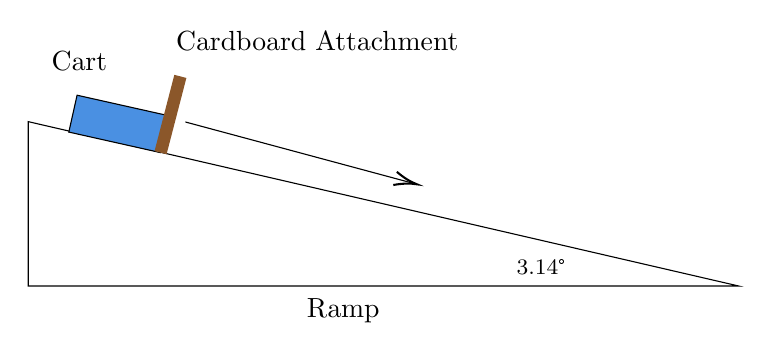
\begin{tikzpicture}[x=0.75pt,y=0.75pt,yscale=-1,xscale=1]
%uncomment if require: \path (0,300); %set diagram left start at 0, and has height of 300

%Shape: Right Triangle [id:dp18569224305294485] 
\draw   (3,189) -- (345.3,268.2) -- (3,268.2) -- cycle ;
%Shape: Rectangle [id:dp7438562411637597] 
\draw  [fill={rgb, 255:red, 74; green, 144; blue, 226 }  ,fill opacity=1 ] (26.54,176.27) -- (70.74,186.17) -- (66.76,203.93) -- (22.56,194.03) -- cycle ;
%Straight Lines [id:da735201395514776] 
\draw [color={rgb, 255:red, 139; green, 87; blue, 42 }  ,draw opacity=1 ][line width=4.5]    (76.3,167.2) -- (66.76,203.93) ;
%Straight Lines [id:da10025482914979356] 
\draw    (78.74,189.17) -- (188.37,218.68) ;
\draw [shift={(190.3,219.2)}, rotate = 195.06] [color={rgb, 255:red, 0; green, 0; blue, 0 }  ][line width=0.75]    (10.93,-3.29) .. controls (6.95,-1.4) and (3.31,-0.3) .. (0,0) .. controls (3.31,0.3) and (6.95,1.4) .. (10.93,3.29)   ;

% Text Node
\draw (237,254) node [anchor=north west][inner sep=0.75pt]   [align=left] {{\fontfamily{}\selectfont {\footnotesize 3.14°}}};
% Text Node
\draw (13,154) node [anchor=north west][inner sep=0.75pt]   [align=left] {{\fontfamily{}\selectfont Cart}};
% Text Node
\draw (73,144) node [anchor=north west][inner sep=0.75pt]   [align=left] {{\fontfamily{}\selectfont Cardboard Attachment}};
% Text Node
\draw (136,273) node [anchor=north west][inner sep=0.75pt]   [align=left] {{\fontfamily{}\selectfont Ramp}};


\end{tikzpicture}
\caption{General experimental setup with a \textit{Smart Cart} rolling down a ramp. Cross-sectional area of the cart is changed using a cardboard attachment.}
\end{figure}

\blindtext %delete this line

\section{Methods}


Give a schematic of the experimental setup(s) used in the experiment (see
figure~\ref{fig:samplesetup}). Give the description of  abbreviations
either in the figure caption or in the text. Write a description of what is
going on. 

%\begin{figure}[ht] 
        % read manual to see what [ht] means and for other possible options
%        \centering \includegraphics[width=0.8\columnwidth]{sr_setup}
        % note that in above figure file name, "sr_setup",
        % the file extension is missing. LaTeX is smart enough to find
        % apropriate one (i.e. pdf, png, etc.)
        % You can add this extention yourself as it seen below
        % both notations are correct but above has more flexibility
        %\includegraphics[width=1.0\columnwidth]{sr_setup.pdf}
%        \caption{
%                \label{fig:samplesetup} % spaces are big no-no withing labels
                % things like fig: are optional in the label but it helps
                % to orient yourself when you have multiple figures,
                % equations and tables
%                Every figure MUST have a caption.
%        
%\end{figure}

and eventually arrived to the
balanced photodiode as seen in the figure~\ref{fig:samplesetup}.


\section{Results}

In this section you will need to show your experimental results. Use tables and
graphs when it is possible. Table~\ref{tbl:bins} is an example.

\begin{table}[ht]
\begin{center}
\caption{Every table needs a caption.}
\label{tbl:bins} % spaces are big no-no withing labels
\begin{tabular}{|cc|} 
\hline
\multicolumn{1}{|c}{$x$ (m)} & \multicolumn{1}{c|}{$V$ (V)} \\
\hline
0.0044151 &   0.0030871 \\
0.0021633 &   0.0021343 \\
0.0003600 &   0.0018642 \\
0.0023831 &   0.0013287 \\
\hline
\end{tabular}
\end{center}
\end{table}

Analysis of equation~\ref{eq:equation1} shows ...

\blindtext

\begin{figure}
    \centering
    \caption{Hyperbolic tangent acceleration vs immediate constant acceleration. The slow approach to the same asymptotic value of 2 meters per second per second induces a lag in the oscillation and also diminishes the amplitude of oscillation.}
\end{figure}

For example, it is easy to conclude that the
experiment and theory match each other rather well if you look at
Fig.~\ref{fig:samplesetup} and Fig.~\ref{fig:exp_plots}.


\section{Conclusions}
Here you briefly summarize your findings. Did you learn any new physics? Was everything as expected?

\blindtext

\section{Future Work}
Since you had limited time to work on this project, what questions are left outstanding? What would be your next steps? 

\blindtext

%++++++++++++++++++++++++++++++++++++++++
% References section will be created automatically 
% with inclusion of "thebibliography" environment
% as it shown below. See text starting with line
% \begin{thebibliography}{99}
% Note: with this approach it is YOUR responsibility to put them in order
% of appearance.

\begin{thebibliography}{99}

\bibitem{melissinos}
A.~C. Melissinos and J. Napolitano, \textit{Experiments in Modern Physics},
(Academic Press, New York, 2003).

\bibitem{Cyr}
N.\ Cyr, M.\ T$\hat{e}$tu, and M.\ Breton,
% "All-optical microwave frequency standard: a proposal,"
IEEE Trans.\ Instrum.\ Meas.\ \textbf{42}, 640 (1993).

\bibitem{Wiki} \emph{Expected value},  available at
\texttt{http://en.wikipedia.org/wiki/Expected\_value}.

\end{thebibliography}


\end{document}